The Medial Triangle divides the plane in 7 regions, see  Figure~\ref{fig:midlines}. The following is a known fact  \cite{akopyan2007-conics,odehnal2015-conics}:

\begin{remark}
If the center of a Circumconic lies within 4 of these (resp. the remainder 3), the conic will be an Ellipse (resp. Hyperbola).
\end{remark}

\begin{figure}
    \centering
    % used inkspace to go from .pdf -> .eps
    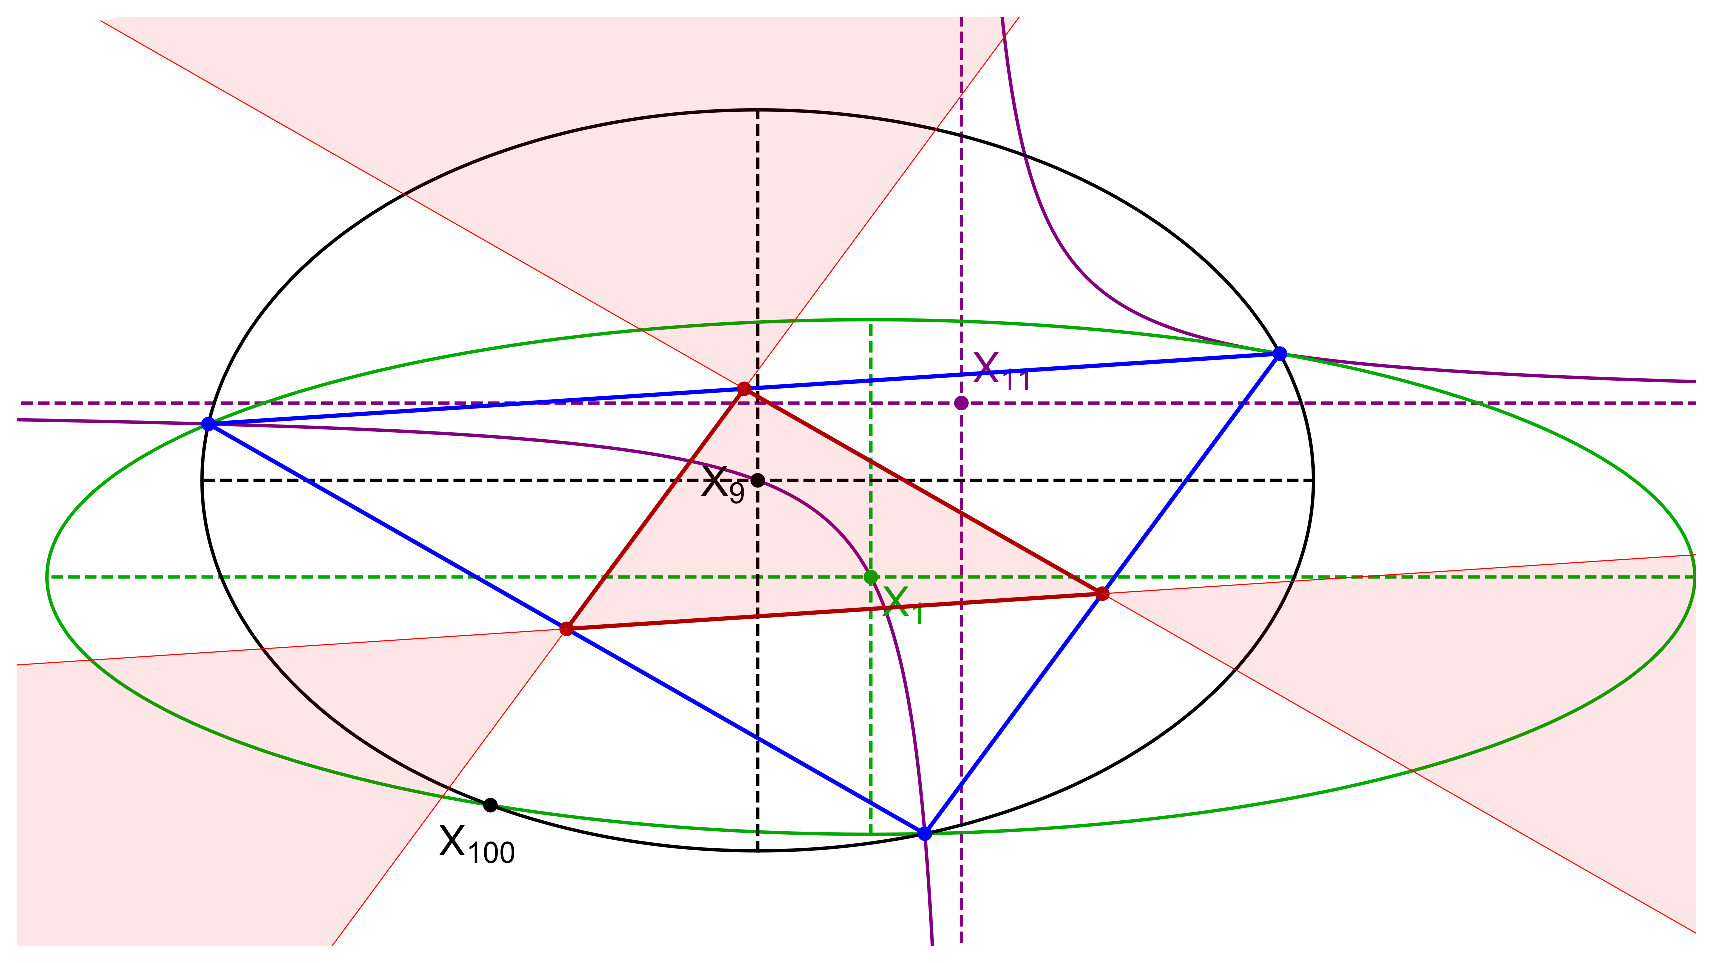
\includegraphics[width=\textwidth]{pics_eps_new/0070_medial_midlines_cropped.eps}
    \caption{A reference triangle is shown (blue) as well as its Medial (red). The latter sides divide the plane into 7 regions, including the Medial' s interior. When a Circumconic center lies on any of the shaded regions (resp. unshaded) it is an Ellipse (resp. Hyperbola). Parabolas have centers at infinity. For illustration, the $X_1$ and $X_9$-centered Circumellipses and the $X_{11}$-centered Feuerbach Hyperbola are shown. Note that over the family of 3-periodics, a given Circumconic may alternate between Ellipse and Hyperbola, e.g., when centered on $X_4$, $X_5$, $X_6$, etc.}
    \label{fig:midlines}
\end{figure}

Centers $X_1$, $X_2$, and $X_9$ are always interior to the Medial Triangle \cite{etc}, so the Circumconics $E_i,i=1,2,9$ centered on them will ellipses, Figure~\ref{fig:circumX1X2}. $E_2$ is the {\em Steiner Circumellipse}, least-area over all possible Circumellipses \cite{mw}, and $E_9$ is $T$'s CB, see Section~\ref{sec:cb}.

It is known that $E_1$ intersects the EB and the Circumcircle at $X_{100}$, the Anticomplement of the Feuerbach Point. Also that $E_2$ intersects $E_9$ at $X_{190}$, the Yff Parabolic Point \cite{dekov14,etc}. These two ellipses intersect at $X_{664}$\footnote{This is the isogonal conjugate of $X_{663}$, i.e., $\mathcal{L}_{663}$ mentioned before is coincidentally its {\em Trilinear Polar} \cite{mw}.} \cite{moses2020-private-circumconic}.

Given a generic triangle $T$:

\begin{proposition}
The axes of $E_1$  are parallel to $E_9$'s. %${e_1}{e_2}={-a^2+2+2\delta}{a^4(2 a^2-1+2\delta)}$.
\end{proposition}

The proof is in Appendix~\ref{app:circum-x1x2x9}. 

\begin{theorem}
Let $\eta_1$ and $\eta_1'$ be the lengths of minor and major semi-axes of $E_1$, respectively. The ratio of their lengths is constant over the 3-periodic family and given by:
\begin{equation*}
\frac{\eta_1'}{\eta_1}=\frac{\sqrt{2\delta^2+2(a^2-b^2)\delta-a^2b^2}}{b^2} >1
\end{equation*}
\label{thm:axis-ratio}
\end{theorem}

%\begin{equation}
%\label{eqn:rovR}
%\frac{r}{R}=\frac{2(\delta-b^2)(a^2-\delta)}{(a^2-b^2)^2}
%\end{equation}

\begin{proof}
Calculate the ratio using vertex locations (see \cite{garcia2020-new-properties}) for an isosceles orbit, and then verify with a Computer Algebra System (CAS) the expression holds over the entire family.
\end{proof}

Note: experimentally $\eta_1'$ is maximal (resp. minimal) when the 3-periodic is an isosceles with axis of symmetry parallel to the EB's minor (resp. major) axis.

\begin{proposition}
The axes of $E_2$ are only parallel to $E_9$ if $T$ is isosceles.
\end{proposition}

See Appendix~\ref{app:circum-x1x2x9}.

%\begin{observation}
%The intersection of %$E_1$ and $E_2$ which is %not a vertex of $T$ is %collinear with $X_{75}$ %and $X_{77}$.
%\end{observation}


% \begin{observation}
%$E_2$ axes are only parallel to the EB's when orbits are isosceles triangles (4 discrete cases). Their lengths $\eta_2$ and $\eta_2'$ are related as $\eta_2 = c_0 + c_1 \eta_2'$, with $c_0,c_1$ constant for all orbits. \textcolor{red}{ronaldo consegue derivar $c_0$ e $c_1$?}
%\end{observation}

\begin{figure}
    \centering
    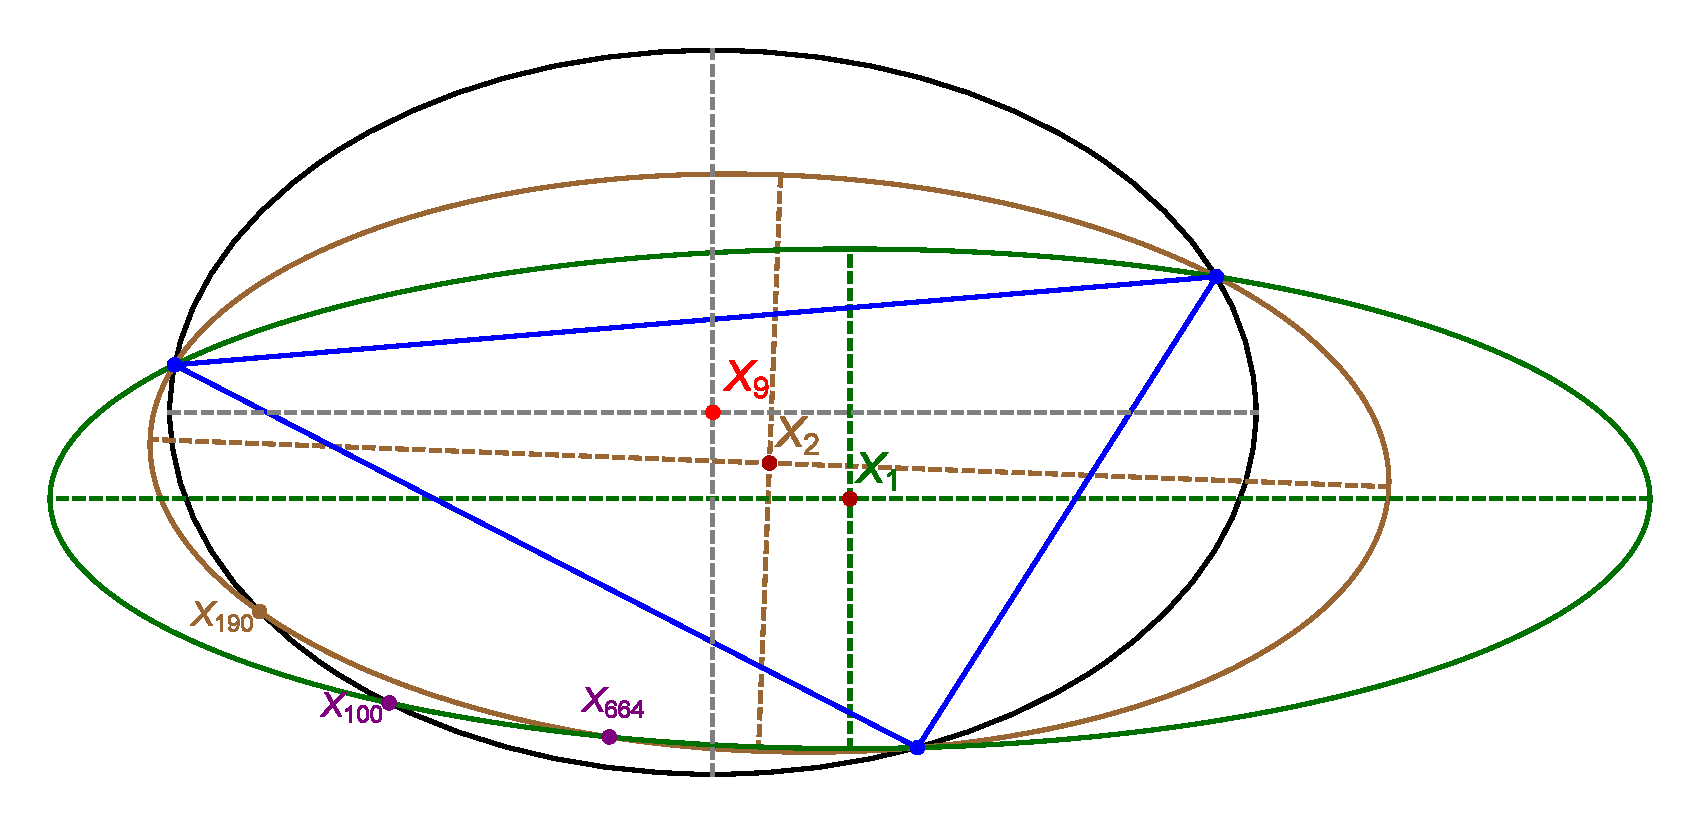
\includegraphics[width=\textwidth]{pics_eps_new/0091_e1e2.eps}
    \caption{$E_1$ (green) and $E_2$ (brown) are Circumellipses to the orbit (blue) centered on $X_1$ (green) and $X_2$ (brown). The former (resp.~latter) intersect the EB at $X_{100}$ (resp.~$X_{190}$). They intersect at the vertices and at $X_{664}$. $E_1$ axes remain parallel to the EB over the orbit family, and the ratio of their lengths is constant. The axes of $E_2$ are only parallel to the EB's when the orbit is an isosceles. \textbf{Video}: \cite[PL\#08]{reznik2020-playlist-circum}.}
    \label{fig:circumX1X2}
\end{figure}

\subsection{Parallel-Axis Pencil}

The Feuerbach Circumhyperbola of a Triangle is a rectangular hyperbola\footnote{Since it passes through the Orthocenter $X_4$ \cite{mw}.} centered on $X_{11}$ \cite{mw}.
Peter Moses has contributed a stronger generalization \cite{moses2020-private-circumconic}:

\begin{remark}
The pencil of Circumconics whose centers lie on the Feuerbach Circumhyperbola $F_{med}$ of the Medial Triangle have mutually-parallel axes. 
\end{remark}

The complement\footnote{The 2:1 reflection of a point about $X_2$.} of $X_{11}$ is $X_{3035}$ \cite{etc} so $F_{med}$ is centered there, see Figure~\ref{fig:circum_parallel}. The following is a list of Circumellipses whose centers lie on $F_{med}$ \cite{moses2020-private-circumconic}: $X_i$,  $i$=1, 3, 9, 10\footnote{Notice $X_{10}$ is the Incenter of the Medial. Interestingly, $X_8$, the Incenter of the ACT, does not belong to this select group.}, 119, 142, 214, 442, 600, 1145, 2092, 3126, 3307, 3308, 3647, 5507, 6184, 6260, 6594, 6600, 10427, 10472, 11517, 11530, 12631, 12639, 12640, 12864, 13089, 15346, 15347, 15348, 17057, 17060, 18258, 18642, 19557, 19584, 22754, 34261, 35204.
%The  results below have been observed experimentally, but still lack a proof.

\begin{proposition}
\label{th:9}
A circumellipse has  center on $F_{med}$ iff it passes through $X_{100}$.
\end{proposition}

A proof appears in Appendix~\ref{app:ce_parallel}. The following has been observed experimentally:

\begin{conjecture}
Over the family of 3-periodics, all Circumellipses in Moses' pencil conserve the ratio of their axes.
\label{conj:moses}
\end{conjecture}

\begin{figure}
    \centering
    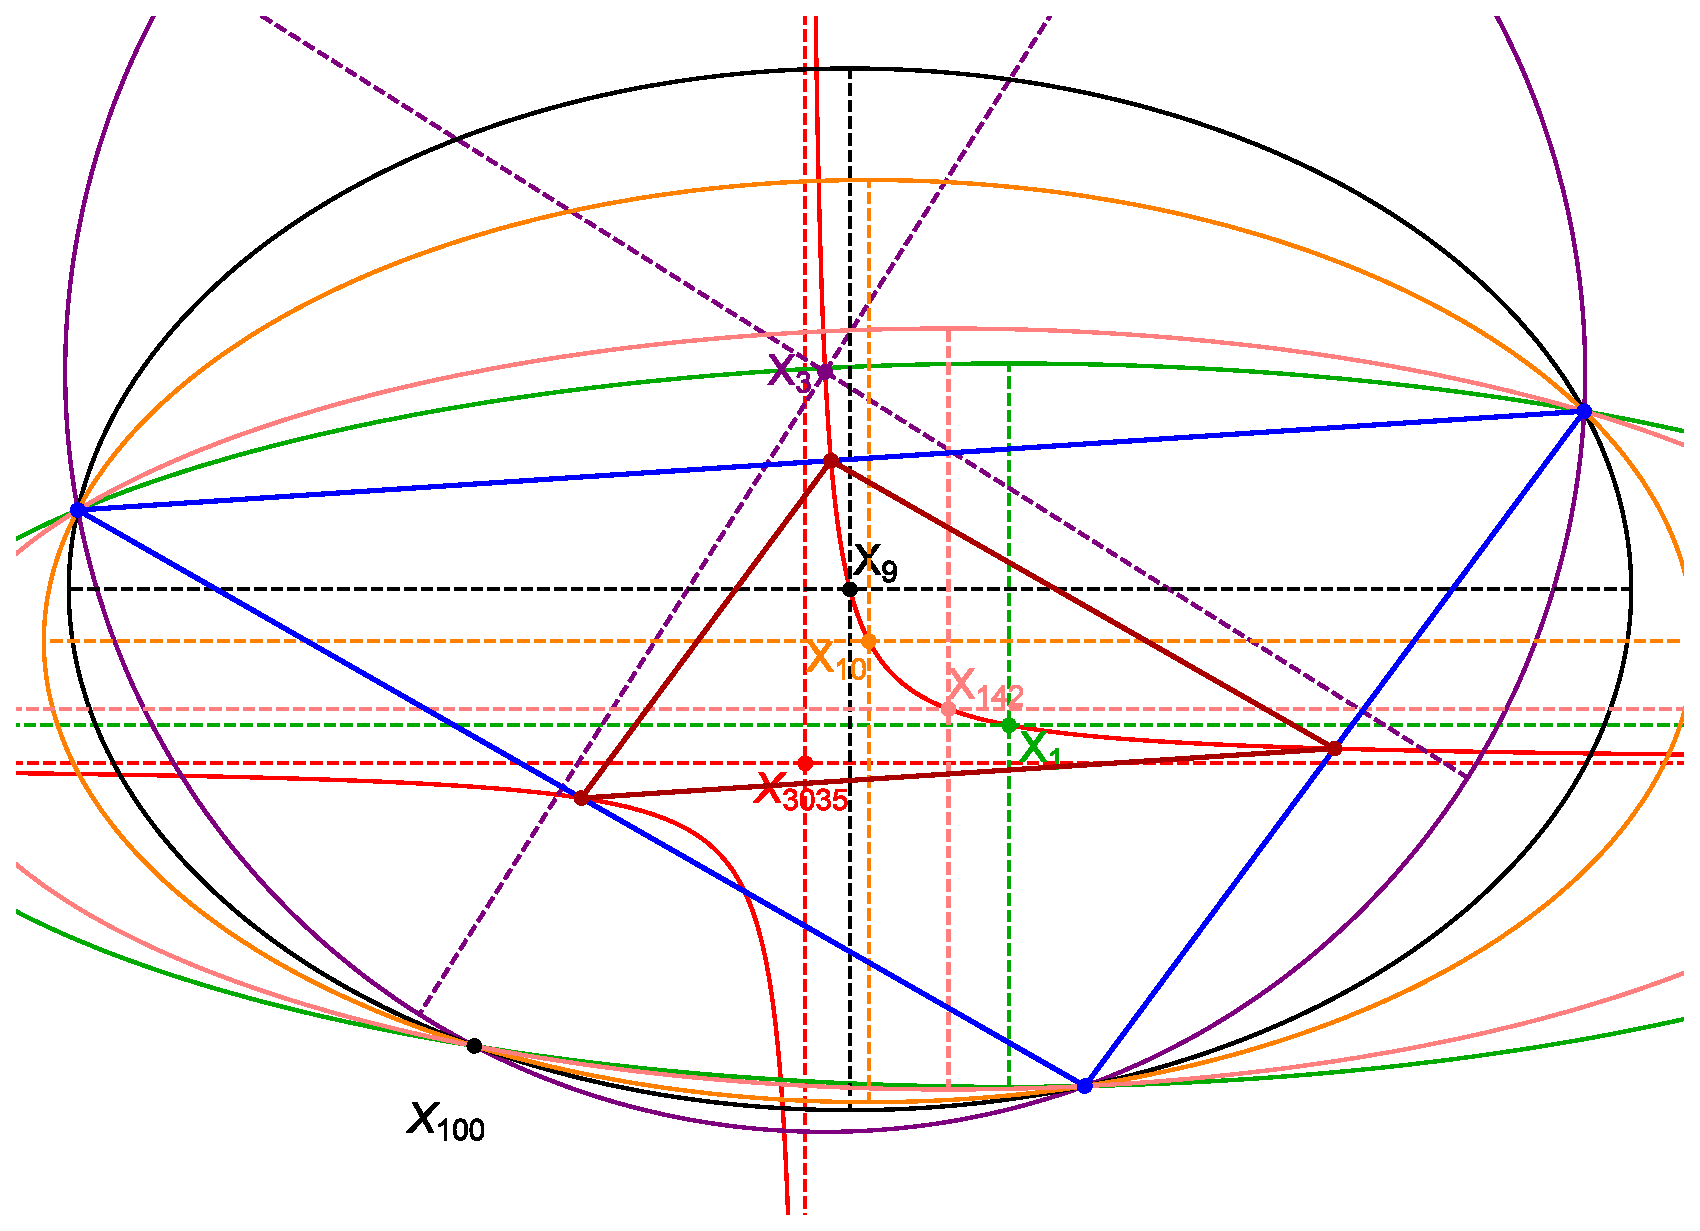
\includegraphics[width=\textwidth]{pics_eps_new/0050_ce_x100.eps}
    \caption{An $a/b=1.5$ EB is shown (black) centered on $X_9$ as well as a sample 3-periodic (blue). Also shown are Circumellipses centered on $X_i$, $i=$1, 3, 10, 142, whose centers lie on the Feuerbach Circumhyperbola of the Medial Triangle (both shown red), centered on $X_{3035}$, the complement of $X_{11}$. Notice all conics drawn (including the Circumhyp). have axes parallel to the EB and all Circumellipses pass through $X_{100}$. Note: the Circumellipse centered on $X_3$ is the Circumcircle, its axes, drawn diagonally, are immaterial.}
    \label{fig:circum_parallel}
\end{figure}